\chapter{Introduction}
\label{sec:introduction}



Since the invention of modern computers, Monte Carlo methods have become an increasingly applied tool for challenging numerical problems in a wide variety of fields ranging from chemical physics to financial econometrics. Although the evolution of computers is proceeding, the complexity of considered problems is growing faster and Monte Carlo methods are now expected to deal with high dimensionalities and more and more complex structures. Hence the efficiency of these methods is also nowadays a crucial question.

In this thesis we present a large subclass of Monte Carlo methods, the Markov chain Monte Carlo (MCMC) methods. The MCMC methodology [Robert,Casella] provides a framework for many algorithms which affect the sampling from complex probability distributions in high dimensions by generating a Markov chain. It is therefore of interest to analyse the structure inherent in these algorithms to understand the computational complexity of MCMC methods. This is most naturally undertaken by studying the behavior of the method on a family of probability distributions indexed by a parameter and studying the cost of the algorithm as a function of that parameter. Therefore diffusion limits of MCMC methods in high dimensions provide
a useful theoretical tool for studying computational complexity. In particular we will study these algorithms applied to a family of probability distributions found from finite-dimensional approximations of a measure on an infinite-dimensional space.


Our interest is focused on Metropolis-Hastings MCMC methods [Robert,Casella]. We study the random walk Metropolis algorithm (RWM) and the Metropolis-adjusted Langevin algorithm (MALA)[Liu and Robert,Casella]. 

Consider a $ \pi^{N} $-invariant Metropolis Hastings–Markov chain $ \{ x^{k,N} \}_{k \geq 1} $ . From the current state $ x $, we propose $ y $ drawn from the kernel $ q(x, y) $; this is then accepted with probability
\begin{equation}
 \alpha .
\end{equation}

Two widely used proposals are the random walk proposal (obtained from
the discrete approximation of Brownian motion)
\begin{equation}
\label{RWM-proposals-simple}
 RWM proposals,
\end{equation}

and the Langevin proposal (obtained from the time discretization of the
Langevin diffusion)
\begin{equation}
\label{MALA-proposals-simple}
 MALA proposals.
\end{equation}

Here $ 2 \delta $ is the proposal variance, a parameter quantifying the size of the
discrete time increment; we will consider “local proposals” for which $ \delta $ is
small. The Markov chain corresponding to proposal (\ref{RWM-proposals-simple}) is the (RWM) algorithm [Metropolis], and the Markov transition rule constructed from the proposal (\ref{MALA-proposals-simple}) is known as the (MALA) algorithm [Robert,Casella].


\subsection*{Statement of the problem}

Look at computational cost of MCMC methods as a function of dimension $ N $.

Optimal Scaling for RWM and MALA for different target distributions.

\subsubsection*{Heuristic argument}

In Figure \ref{fig:3DscatterplotRWM}, the opitimal scaling of the acceptance probability and therefore the scaling of the proposal variance is illustrated by a Random Walk Metropolis-Hastings algorithm. A too small proposal variance and therefore a too high acceptance probability causes a very slow mixing of the Markov chain in the two modes of the target density. In the case of a too high proposal variance, the Markov chain stays very long in one state. Hence the efficiency of the algorithm is relatively low.


\begin{figure}[htb]
 \begin{center} 
  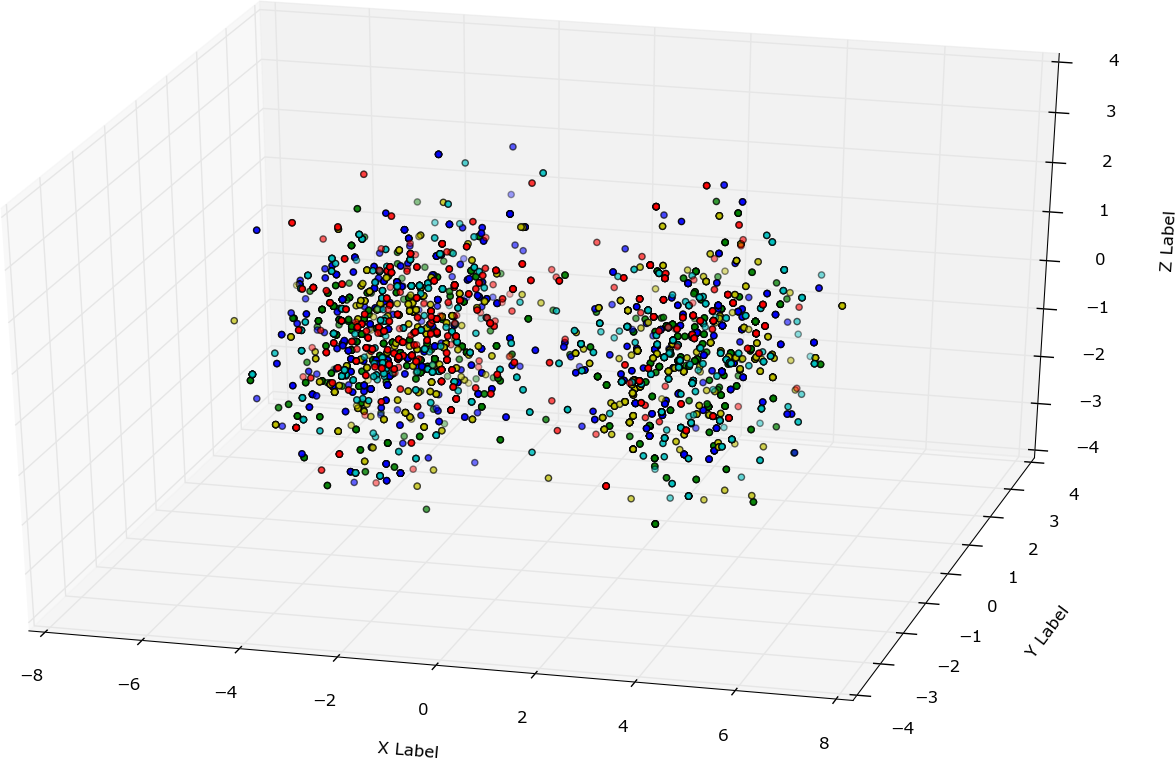
\includegraphics[width=0.56\textwidth]{figure_1}
  \vspace*{1mm}
  \subcaption{Optimal scaled acceptance probability with a good mixing between both modes.}
  \vspace*{3mm}
  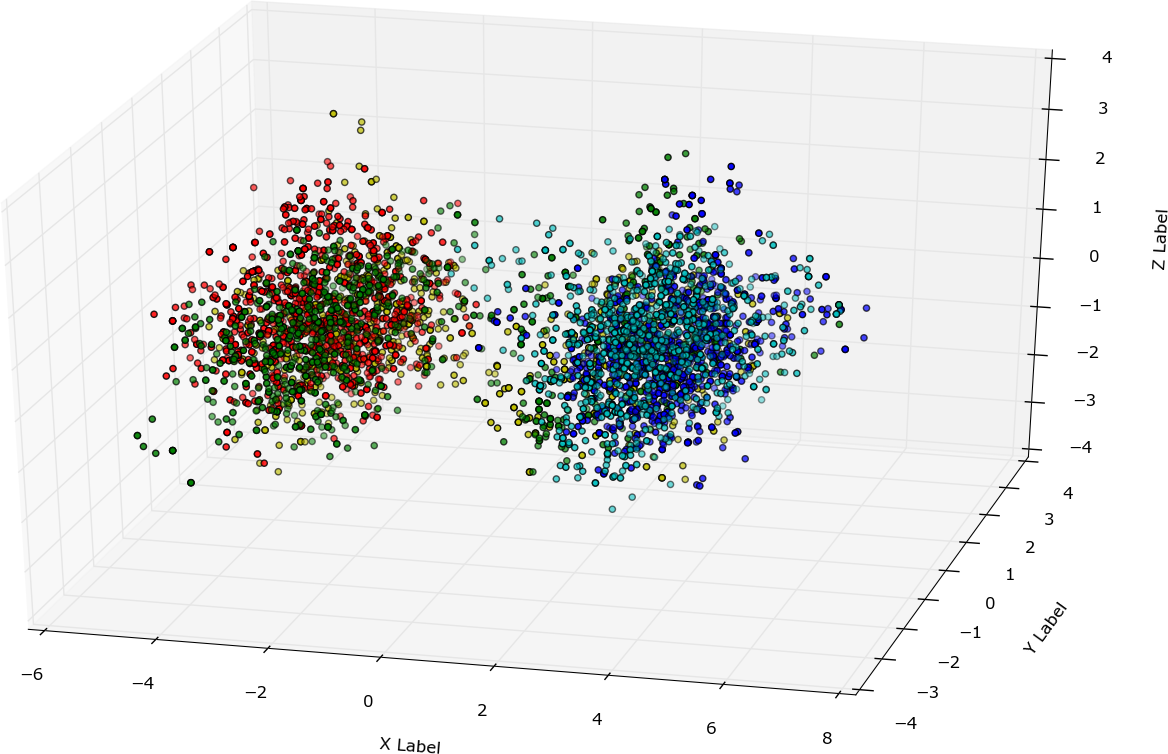
\includegraphics[width=0.55\textwidth]{figure_2}
  \vspace*{1mm}
  \subcaption{Too large acceptance probability with a bad mixing between both modes.}
  \vspace*{3mm}
  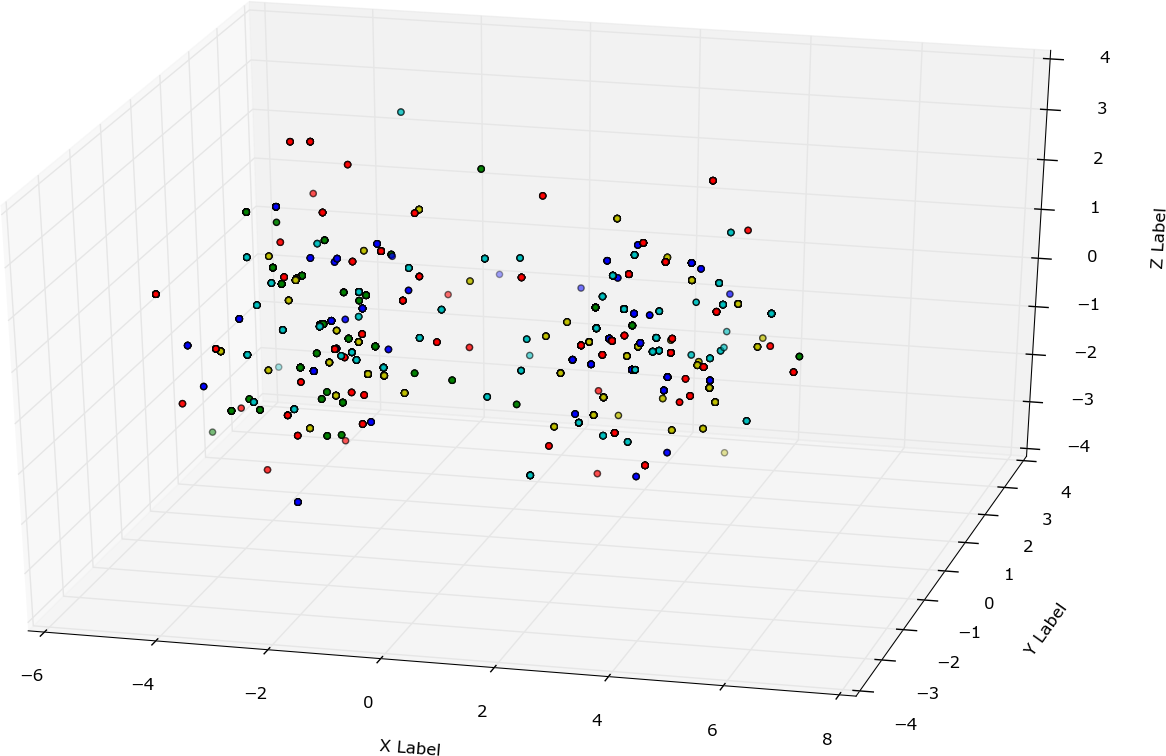
\includegraphics[width=0.55\textwidth]{figure_3}
  \vspace*{1mm}
  \subcaption{Too low acceptance probability.}
 \end{center}
  \caption{5000 samples produced by a RWM algorithm of a multimodal non-product target density. Every 1000 consecutive samples are labeled in the same colour.}
  \label{fig:3DscatterplotRWM}
\end{figure}


\subsection*{Overview}

Give an overview of present results of optimal scaling: Roberts and Rosental, Bedard, Breyer and Piccioni and Scarlatti, Mattingly and Pillai and Stuart and Thiery

\subsection*{Own contributions}

My contributions to the present topic.
\begin{itemize}
 \item First point.
 \item Second point.
 \item Last point.
\end{itemize}


\subsection*{Outline}

A brief outline of the structure of this work.


\subsection*{Acknowledgements}

A list of persons, who deserve my acknowledgements: advisor, parents, friends.



